\documentclass{article}

\usepackage[utf8]{inputenc}
\usepackage{ctex}
\usepackage{assignpkg}
\usepackage{amsmath}
\usepackage{amssymb}

\usepackage{geometry}
\geometry{a4paper,scale=0.8}

% packages drawing picture
\usepackage{tikz}

\studentIds{202XX80XXXXXXXX}{}
\studentNames{XXX}{}

\assignmentNumber{3}

\date{\today}

\begin{document}

\makecover

%\section*{1}
\subsection*{1.试析随机森林为何比决策树 Bagging 集成的训练速度更快;}
  决策树的生成过程中,最耗时的就是搜寻最优切分属性;随机森林在决策树训练过程中引入了随机属性选择,大大减少了此过程的计算量;因而随机森林比普通决策树Bagging训练速度要快。

\subsubsection*{2. 试比较 Gradient Boosting 与 AdaBoost 的异同;}
Gradient Boosting和其它Boosting算法一样,通过将表现一般的数个模型(通常是深度固定的决策树)组合在一起来集成一个表现较好的模型。抽象地说,模型的训练过程是对一任意可导目标函数的优化过程。通过反复地选择一个指向负梯度方向的函数,该算法可被看做在函数空间里对目标函数进行优化。因此可以说Gradient Boosting = Gradient Descent + Boosting。

和AdaBoost一样,Gradient Boosting也是重复选择一个表现一般的模型并且每次基于先前模型的表现进行调整。不同的是,AdaBoost是通过提升错分数据点的权重来定位模型的不足而Gradient Boosting是通过算梯度(gradient)来定位模型的不足。因此相比AdaBoost, Gradient Boosting可以使用更多种类的目标函数。

\subsection*{3. 试比较包裹式选择、过滤式选择与嵌入式选择的异同;}
• 过滤式特征选择方法:

– 先对数据集进行特征选择, 然后再训练分类器;特征 选择过程与分类单独进行, 特征选择评价判据间接反 应分类性能。

— 与包裹式选择方法相比,计算量降低了很多;

• 包裹式特征选择方法:

– 特征选择过程与分类性能相结合, 特征评价判据为分 类器性能。 为给定分类方法, 选择最有利于其性能的 特征子集。

– 直接以分类性能为准则的特征选择方法

• 嵌入式特征选择方法:

– 将分类器学习与特征选择融为一体, 分类器训练 过程自动完成了特征选择。
\subsection*{4. 试述直接求解 L0 范数正则化会遇到的困难;}
$L_0$范数等于非零元素的个数。考虑二维的情况,此时的等值线比较特殊:在原点,$L_0$=0; 在各个坐标轴上$L_0$=1; 在各个象限区域,$L_0$=2。

\begin{tikzpicture}
	\draw[-latex] (-2,0) -- (2,0);
	\draw[-latex] (0,-2) -- (0,2);
	\node() at (1,1) {2};
	\node() at (-1,1) {2};
	\node() at (1,-1) {2};
	\node() at (-1,-1) {2};
	\node() at (0,1) {1};
	\node() at (1,0) {1};
	\node() at (0,-1) {1};
	\node() at (-1,0) {1};
	\node() at (0,0) {0};
	\node() at (0,-2.2) {二维情况下的$L_0$范数};
\end{tikzpicture}


在二维情况下求解$L_0$正则下的回归问题可能是按照如下进行分类讨论:
\begin{itemize}
\item[a]
不限定$\omega$是否存在0值,求解均方误差最小对应的$\omega$。
\item[b]
限定$\omega$中有一0值,求解均方误差最小对应的$\omega$。这种情况有两种。
\item[c]
令$\omega$中为全0值,求解最小均方误差。
\end{itemize}

比较上述所求的最小均方误差。取其中最低的最小均方误差对应的$\omega$。

通过如上所述,我们不难得出,在求解$L_0$正则化问题时,我们需要依次讨论$\omega$中0元素的个数以及分别是哪几个,对于每种情况求解出最小均方误差,再对$\omega$进行取舍。那么这样对于有$N$个特征的问题,则将讨论$2^N$总情况。这个复杂度随特征数指数增长,计算量大,比较困难。
\subsection*{5. 试述为什么基于 L1 范数可以进行特征选择;}
因为最小化$L_1$范数可以得到稀疏解,所谓稀疏解,就是解$\omega$中的零元素相对较多,非零元素则相对较少。而$\omega$中的零元素表示不需要用到对应的特征,只用到了非零元对应的特征。故可进行特征选择。

那么我们来看看为何最小化$L_1$范数可以得到稀疏解。以二维平面的线性回归为例,线性回归求解出来的模型是一条直线(绿线),而$L_1$范数等值线为一系列的以原点为中心,坐标轴为对角线的菱形(如图中的蓝线和红线)。

并且这条直线将与这个棱形存在一个“切点”,可以看到当切点为正方形的顶点时,所得的解是存在0元素的。而若使用$L_2$范数进行求解的话,$L_2$范数的形状表现为一个圆形,直线与圆相切时,只有在极少数情况下才会存在包含0元素的解。所以$L_2$范数将不具有解的稀疏性。
推广至多维的情况,$L_1$范数将是类似于八面体这样具有尖点的形状,而$L_2$范数将是球状。两者仍然具有以上的性质,故$L_1$范数更能得到稀疏解。

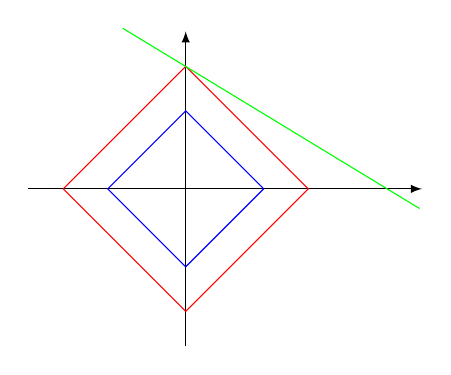
\begin{tikzpicture}
	\draw[-latex] (-2,0) -- (3,0);
	\draw[-latex] (0,-2) -- (0,2);
	\draw[rotate=45, blue] (-0.7,-0.7) rectangle (0.7,0.7);
	\draw[rotate=45,color=red] (-1.1,-1.1) rectangle (1.1,1.1);
	\draw[green] (-0.8, 2.04) -- (2.97,-0.25);
\end{tikzpicture}

\subsection*{6. 试比较 K-SVD 与 K-means 方法的异同;}

• 相同

- K-SVD算法是求解字典学习的常用算法,K-SVD算法是K-means聚类算法的推广形式,即两个都可以看作是字典学习算法,可以从字典学习的角度去理解它们。

- 都可用于聚类

• 不同

– 从字典学习的角度来看K-means聚类算法,通过最近邻来寻找数据点的最优表示字典,数据点的稀疏编码仅有一个非零值

– 而K-SVD算法作为一般的字典学习算法,数据点的稀疏编码有多个非零值

- 相比于K-Means,K-SVD还可用于编码、压缩

\end{document}
